\documentclass[10pt]{article}
\usepackage[pdftex]{graphicx}
\graphicspath{{./images/}}
\usepackage{amsmath,amssymb}
\usepackage{dirtytalk}
\usepackage{anyfontsize}
\usepackage{xcolor}
\usepackage{hyperref}
\hypersetup{
    colorlinks,
    linkcolor={red!50!black},
    citecolor={blue!50!black},
    urlcolor={blue!80!black}
}
\usepackage[skip=10pt plus1pt, indent=40pt]{parskip}
\usepackage{../../common_styles/csagh}


\begin{document}
\begin{opening}
  \title{Logistic regression with Python}
  \author[Universidad Autónoma de Nuevo León, San Nicolás de los Garza, aldo.hernandezt@uanl.edu.mx]{Aldo Hernández}

  \keywords{...}
  \begin{abstract}
    Logistic regression is a supervised algorithm that classifies data into given classes based on their information, it uses the $L_{2}$ function for minimizing loss and converges to a minimum-error solution even if data is not linearly separabale. This document is an introduction to said process while analyzing a real dataset using Python. To do this, we explore the mathematical definitions around this method, use Python code to analyze data and create a logistic regression model to make predictions based on this data. Our conclusions indicate that this type of model is suitable for classification of any dataset using a cross validation method, since it removes the overfitting problem that is naturally found in this type of classification.
  \end{abstract}

  \keywords{logistic regression, python, model, machine learning}
\end{opening}

\section{Introduction}
Linear functions can be used not only for regression, but also for \textbf{classification}. In this case, the line---or surface---is called a \textit{decision boundary}---also known as linear separator---and the data that admits this separator are called \textit{linearly separable}. \cite{ai} In order to use these functions for classification, the first approach was to use the $threshold$ function as the classification hypothesis
\begin{equation*}
  h_{w}(x) = Threshold(w \cdot x) \text{ where } Threshold(z) = 1 \text{ if } z \geq 0 \text{ and } 0 \text{ otherwise}
\end{equation*}
\begin{equation} \label{eq:1}
  w_{i} \leftarrow w_{i} + \alpha (y - h_{w}(x)) \times x_{i}
\end{equation}
But this method has some pretty big disadvantages: even though it is \textit{guaranteed} to converge with linearly separable data, it may take too many steps to do so, also, data may not be linearly separable always, so the algorithm (weight update rule shown in Equation \ref{eq:1}) will fail to converge for a fixed learning rate $\alpha$, unless it decays as $O(1/t)$ where $t$ is the iteration number, then it is shown to converge to a minimum-error solution. \cite{ai} \par
Also, the hypothesis is not differentiable and is a discontinuous function of its inputs and weights, which makes learning with the \textbf{perceptron rule} shown in Equation \ref{eq:1} pretty complicated. Besides, this function will always return a confident prediction of 1 or 0, even if examples are too close to the boundary; in a lot of situations, this is not optimal since we will need more gradated predictions. \cite{ai} \par
It's because of these issues that \textit{logistic regression} surges as a better alternative. We define a function---known as logistic or sigmoid---as follows
\begin{equation*}
  h_{w}(x) = Logistic(w \cdot x) = \frac{1}{1 + e^{-w \cdot x}}
\end{equation*}
This hypothesis gives a probability of $0.5$ for every input at the center, and approaches 0 or 1 as we move away from the boundary \cite{ai}. The process of fitting the weights to this model to minimize the loss on a dataset is called \textbf{logistic regression} \cite{ai}, there is no easy closed-form solution to find the optimal value of $w$ but gradient descent computation is straightforward. Partially differentiating the $L_{2}$ function we get the following
\begin{equation*}
  \frac{\partial}{\partial w_{i}}(y - h_{w}(x))^{2} = -2(y - h_{w}(x)) \times h_{w}(x)(1 - h_{w}(x)) \times x_{i}
\end{equation*}
Thus, the weight update for minimizing the loss is
\begin{equation*}
  w_{i} \leftarrow w_{i} + \alpha(y - h_{w}(x)) \times h_{w}(x)(1 - h_{w}(x)) \times x_{i}
\end{equation*}
This process is a \textbf{supervised algorithm} that can classify data into two states---binary, as shown earlier---or multiple tags \cite{aprendeML}. Some common use cases are:
\begin{itemize}
  \item Classify mail into spam or not.
  \item Classify tumors into benign or malignant.
  \item Classify the content of an article.
\end{itemize}

\section{Methodology}
\subsection{Before typing code} \label{sub:beforeanycode}
First of all, we need to download this \href{http://www.aprendemachinelearning.com/wp-content/uploads/2017/11/usuarios_win_mac_lin.csv}{.csv file} \cite{aprendeML} from where we will obtain our dataset, this file has information about users that visit a certain website, such as: visit duration, viewed pages, total actions made, action value sum, and operating system---0 for Windows, 1 for MacOS, and 2 for Linux---. Next, we will import some necessary libraries to our script
\begin{figure}[h]
  \centering
  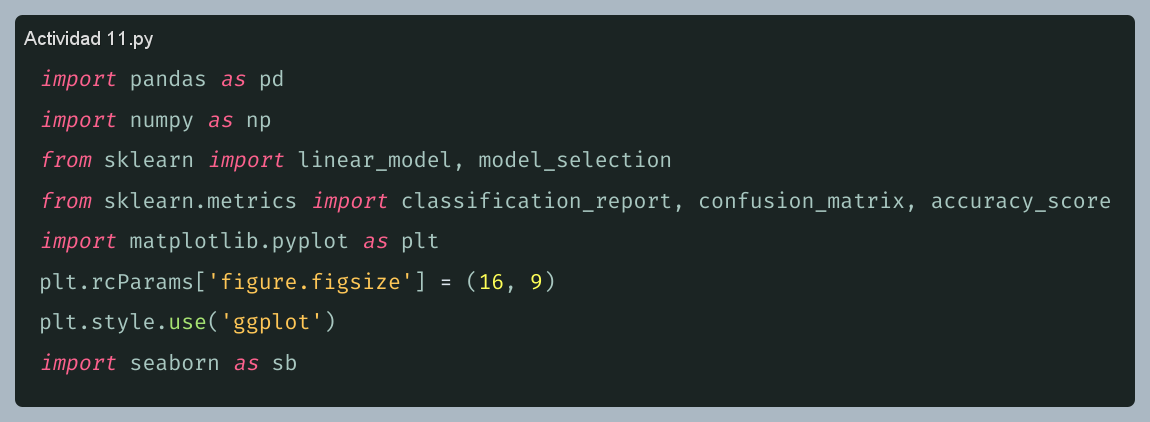
\includegraphics[width=90mm]{./images/2025-03-28-08-55-18.png}
  \caption{Necessary library imports.}
\end{figure}

\subsection{Data analysis}
Next, let's analyze our data, we will parse it from the .csv file we downloaded in Subsection \ref{sub:beforeanycode}, and then print out some useful information \par
\begin{figure}[h]
  \centering
  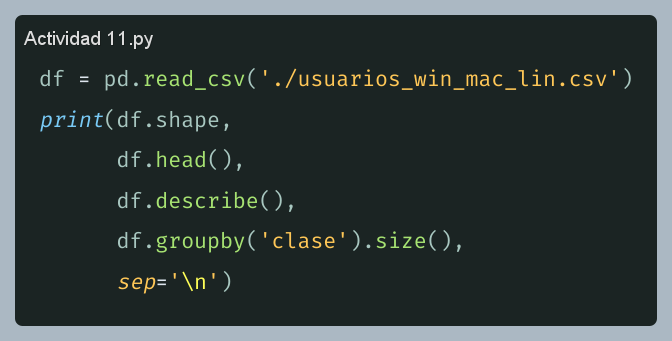
\includegraphics[width=90mm]{./images/2025-03-28-08-59-30.png}
  \caption{Displaying information about the dataset.}
  \label{fig:data_info}
\end{figure}
Thanks to these lines of code, we know that there are 170 rows of data along 5 columns, where 86 rows are Windows users, 40 are MacOS users, and 44 are Linux users. Besides, we may find the following information useful for further analysis \par
\begin{table}[!ht]
  \centering
  \caption{Column information}
  \label{tbl:col_info}
    \begin{tabular}{|c|c|c|c|c|}
      \hline
       & Duration & Pages & Actions & Value \\
      \hline
      Count & 170 & 170 & 170 & 170 \\
      \hline
      Mean & 111.08 & 2.04 & 8.72 & 35.68 \\
      \hline
      Std & 202.45 & 1.50 & 9.14 & 44.75 \\
      \hline
    \end{tabular}
\end{table}
\newpage
After this quick review, we will create a lot of graphs in order to understand the information \par
\begin{figure}[h]
  \centering
  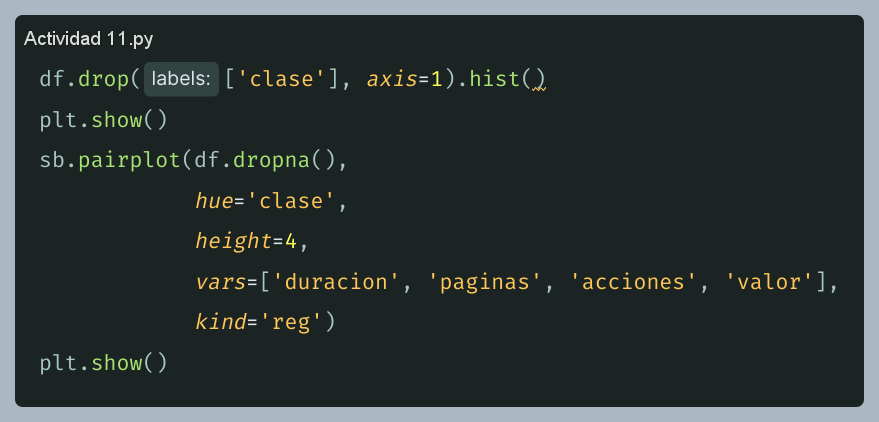
\includegraphics[width=90mm]{./images/2025-03-28-09-56-00.png}
  \caption{Creating histograms and regression plots.}
\end{figure}
\begin{figure}[h]
  \centering
  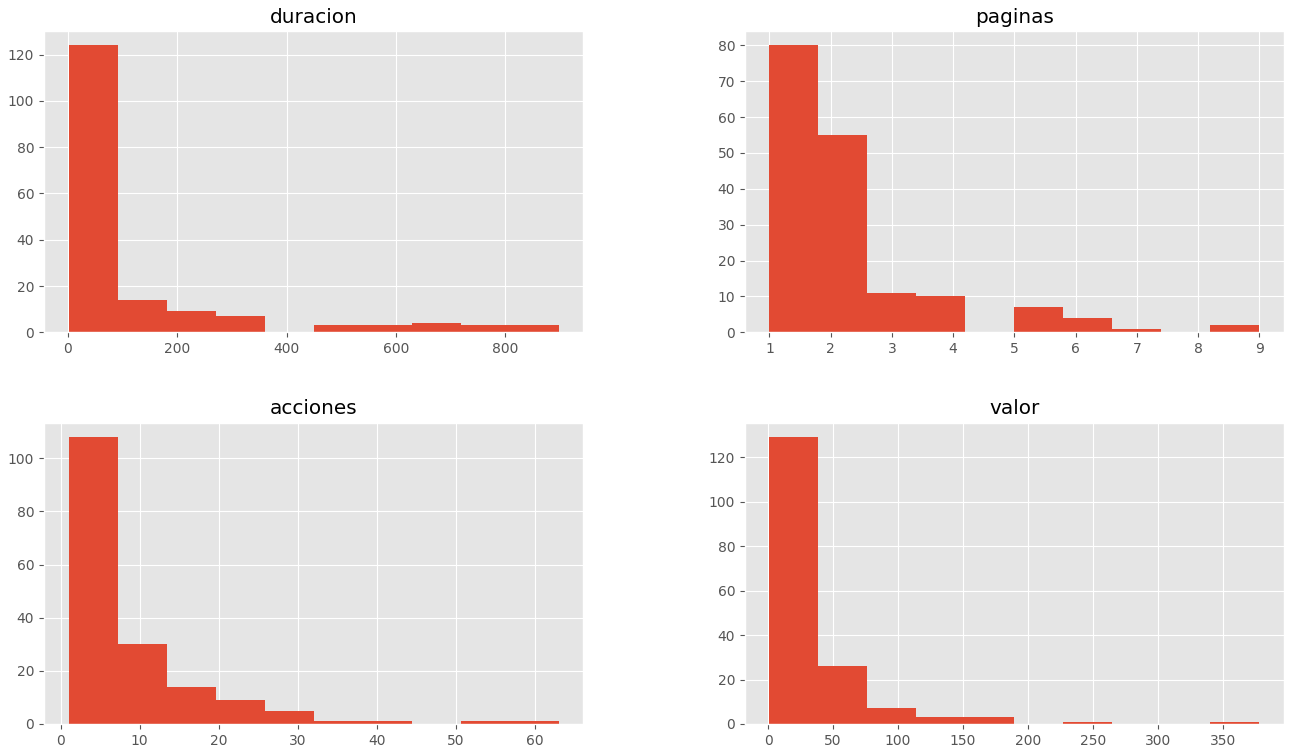
\includegraphics[width=90mm]{./images/2025-03-28-09-59-15.png}
  \caption{Number of rows per column value histograms.}
  \label{fig:hist}
\end{figure}
\begin{figure}[h]
  \centering
  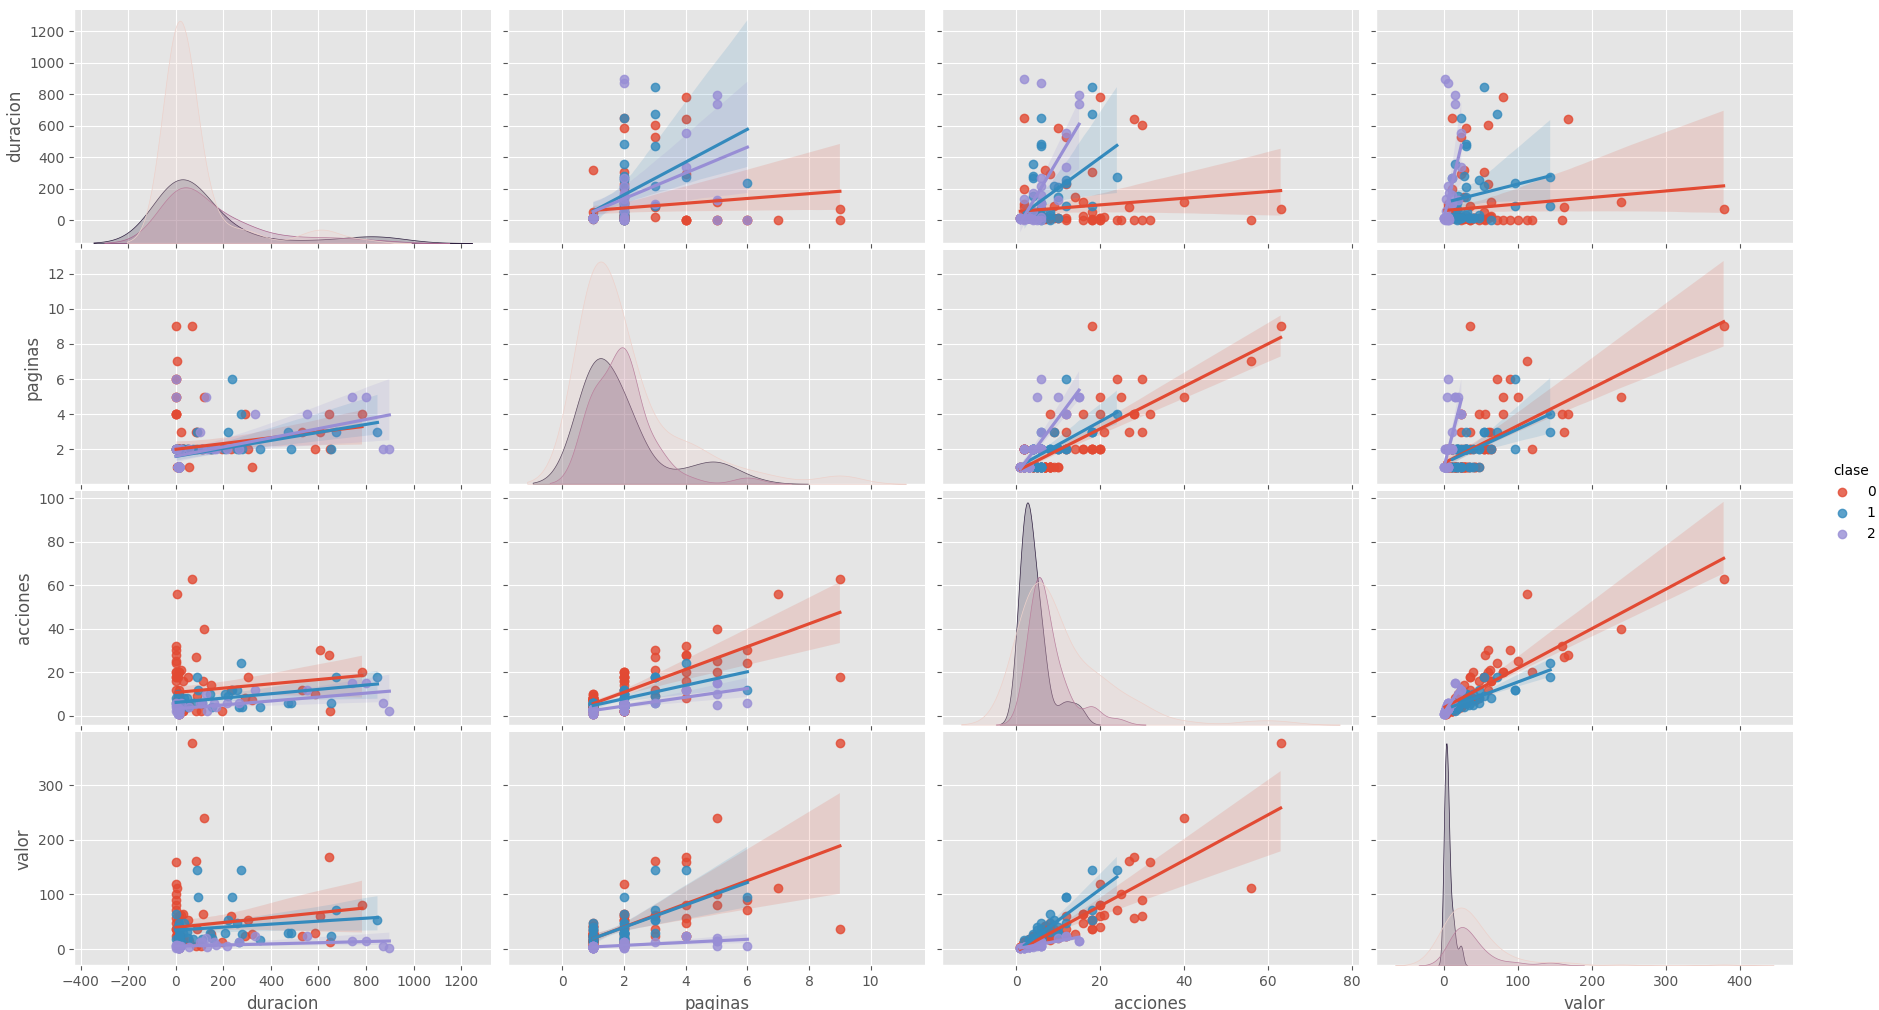
\includegraphics[width=130mm]{./images/2025-03-28-10-02-08.png}
  \caption{Data regression plots.}
  \label{fig:regplots}
\end{figure}
\newpage
From Figure \ref{fig:hist} we can see that duration is mostly concentrated around 0 ms to 100 ms, pages between 1 and 2, actions around 0 to 10, and sum value between 0 to 50. We can also see in Figure \ref{fig:regplots} the lineal relationships between inputs, i. e. MacOS and Linux users do more actions when they spend more time in the website, which may hint that the website has relation with UNIX-like operating systems.

\subsection{Creating the model}
Next, we will create our logistic regression model and print some predictions using training data along with scoring \par
\begin{figure}[h]
  \centering
  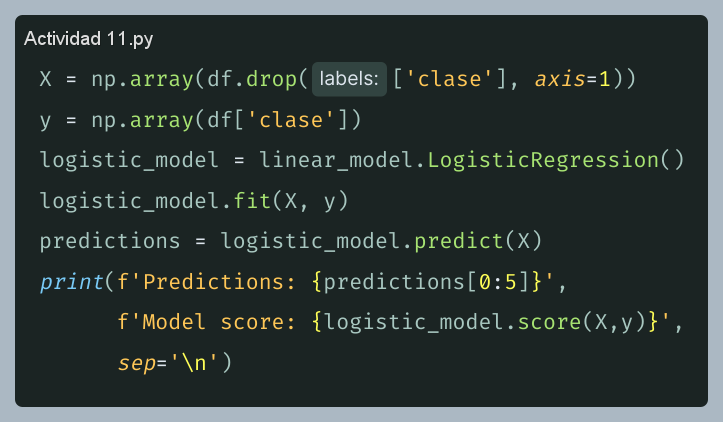
\includegraphics[width=90mm]{./images/2025-03-28-10-19-02.png}
  \caption{Model creation.}
\end{figure}
Turns out that the mean accuracy between predictions and real values is around 71\%, which is a pretty good score.

\subsection{Model validation}
A good practice in machine learning is to divide the dataset into two sets: a training set and a validation set, since this will avoid overfitting problems. \cite{aprendeML} In order to do this, we will use 80\% of the dataset for training and 20\% for validation, said rows will be randomly selected. \par
\begin{figure}[h]
  \centering
  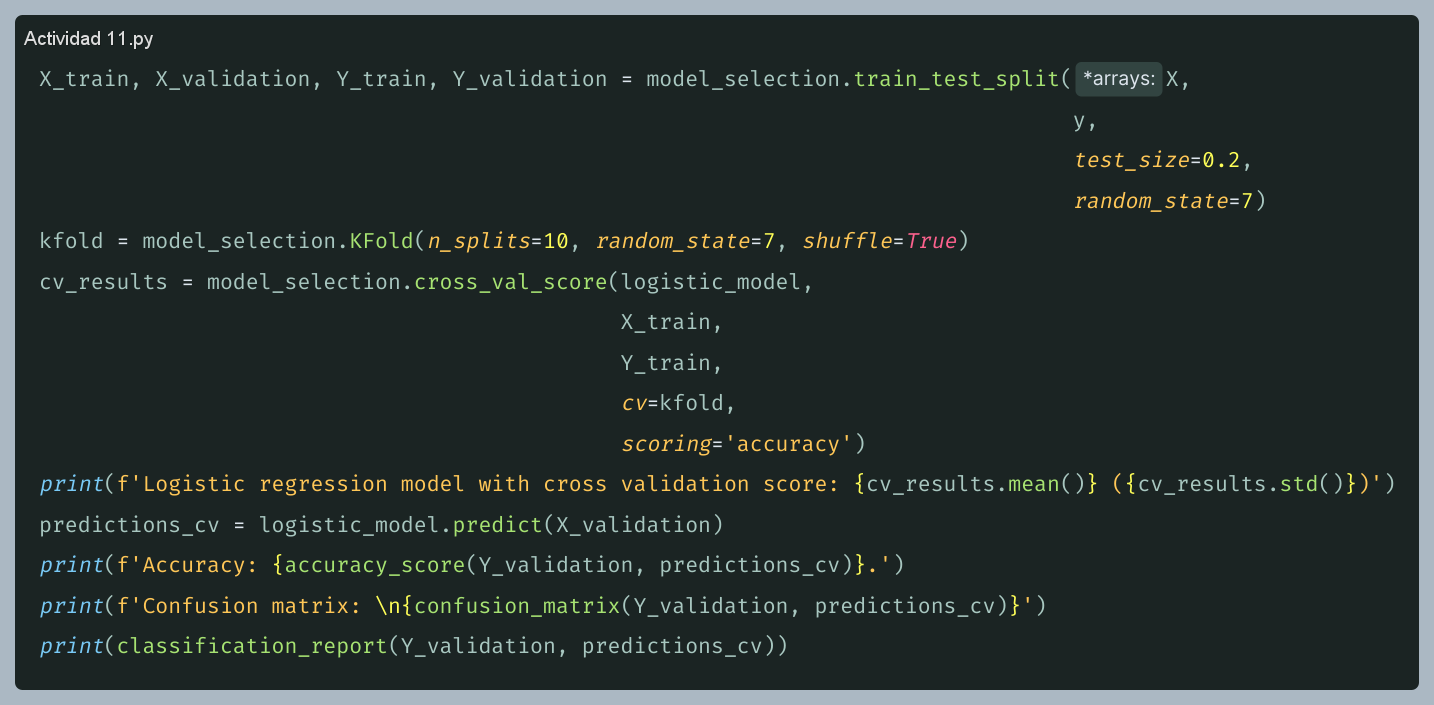
\includegraphics[width=90mm]{./images/2025-03-28-12-24-44.png}
  \caption{Re-compiling the model using only the training set (80\%).}
\end{figure}
Now that we recompiled the model using cross-validation, we make new predictions to test the accuracy, resulting in an 85.29\% accuracy. We also print out the confusion matrix \par
\begin{equation*}
  \left(
    \begin{matrix}
      16 & 0 & 2 \\
      3 & 3 & 0 \\
      0 & 0 & 10
    \end{matrix}
  \right)
\end{equation*}
This matrix tells us that in our predictions, there were 3 real MacOS users predicted as Windows users, and 2 real Windows users predicted as Linux users. We can also see the classification report with our validation set in Table \ref{tbl:classif_report}, that tells us that i. e. MacOS classes had 3 bad predictions and 3 good predictions our of 6 cases (support), the model obtained a 84\% in f1-score, which is a very good value for said metric. 
\begin{table}[!ht]
  \centering
  \caption{Classification report}
  \label{tbl:classif_report}
    \begin{tabular}{|c|c|c|c|c|}
      \hline
       & Precision & Recall & f1-score & Support \\
      \hline
      0 & 0.84 & 0.89 & 0.86 & 18 \\
      \hline
      1 & 1.00 & 0.50 & 0.67 & 6 \\
      \hline
      2 & 0.83 & 1.00 & 0.91 & 10 \\
      \hline
      Weighted avg & 0.87 & 0.85 & 0.84 & 34 \\
      \hline
    \end{tabular}
\end{table}

\section{Results}
Finally, we can make some predictions with this model. For example, let's say a new user visited the website with the following data: \par
\begin{itemize}
  \item Had a duration of 10 seconds.
  \item Visited 3 pages.
  \item Had 5 actions while navigating.
  \item Had a value of 9.
\end{itemize}
Then, the model classifies it as a Linux user.

\section{Conclusions}
After using cross validation to improve our logistic regression model, we obtained a high score even when our sample was small. We conclude that logistic regression models classification is very good, even if the dataset is not so big. Cross-validation improved the model because it removed the overfitting problem we had when first using the whole dataset as training set.

\bibliographystyle{../common_styles/cs-agh}
\bibliography{act11_bibliography}

\end{document}